\input{style.sty}

\begin{document}
	
	\title{Health Care Bot}
	\course{Decision Support Systems}
	\author{Emirhan \textsc{Kutlu}, Lucie \textsc{Labadie}, Rosen \textsc{Sasov}}
	\supervisor{Lawrence \textsc{Henesey}}
	\school{Blekinge Institute of Technology}
	\place{Karlskrona, Sweden}
	\abstractText{In this project we aimed to create a knowledge-based decision support system working in the field of medicine or more specifically in the field of diagnosis making. Our goal was making a system, which provided with symptoms and users personal information as an input data, has the ability to give a final adequate and precise enough suggestion of disease and following treatment. We decided to develop a chatbot having those functionalities.	The chatbot is made to be used only as a helping tool for medical experts and as an informational tool for users and it should have good user interface design.	The system should NOT be used as a tool, that can be trusted completely and blindly, replacing the medical experts expertise. }%TODO
	
	\maketitle
	
	\newgeometry{hmargin=2.5cm,vmargin=2.5cm}
	
	\tableofcontents
	
	\addcontentsline{toc}{chapter}{Introduction}
	\chapter*{Introduction}
	\paragraph{}
	In this project we aimed to create a knowledge-based decision support system working in the field of medicine or more specifically in the field of diagnosis making.\\
    Today a lot of those systems exist but we all know that they have a bad reputation because of their poor decision-making mechanism. Most of us, as users, have tried to check our symptoms and receive a diagnosis using some of those web tools. The result from those tools is more often disappointing rather than convenient. In other words most of the time the diagnosis made is concerning some deadly disease like cancer.\\
	That’s the system that we don’t want to create.\\ 
	Our goal was making a system, which provided with symptoms and users personal information as an input data, has the ability to give a final adequate and precise enough suggestion of disease and following treatment. We want to make a system that helps people go to the right place to be taken care of fast and such that helps for better auto-medication.
	We decided to achieve this with creating a bot based decision support system.\\  
	The first thing that took a lot of time for us was deciding the data model and database structure, that are going to be used.\\
	Our idea is as an input for the bot to use not only symptoms but also some other important side factors as height, weight, age and habits. Taking in consideration those factors is making the final decision more precise. \\
	For the bot we also created a classifier using python scikit-learn for text analysis and natural language processing. The classifier guarantees us a written language recognition and gives us the feature to classify the complaints written as a message by the user.\\ 
	The decision-making strategy is based on decision tree. With every given answer connected to a symptom the possible set with diseases is reducing until we have small enough set which can guarantee us decision with good precision. If there is equality the user personal data gathered at the beginning about age, height, weight and habits is used to determine the final decision. \\
	Along with the decision our bot is providing the user with advice about treatment. At this stage of the project we have 3 categories of advices :
	“Self-treatment” ; “Visit your doctor” and “Go to ER”. \\
	For the logic in the bot we are using Telegram Bot. 
	%TODO
	
	\chapter{Project Analysis} 

\section{Problem definition}

\paragraph{}
Today, the health data that we can access through the internet is quite large. However, due to the data pollution in this area, people may think that they are	caught	in	a	deadly	illness when	they	search	for	a	complaint	they	are	experiencing	on	the	internet.	Even	diseases	that require	long-term	examination	and	detailed	analysis	to	be	diagnosed	can	easily	be	presented to	people.	What's	more,	there	are	many	forums	that	bring	doctors	and	people	together	on	the	internet,	as	well	as	sites	that	function	as	an	individual	dialogue.	On	these	pages,	people	can	ask	irrelevant	or	absurd	questions	to	doctors	because	of	wrong	information	or	ignorance. 

\section{Decision Support System}

\paragraph{}
As our decision making is based on the database, so the facts we possess we can say that our Decision Support System is knowledge-driven. Thanks to out Telegram Bot use, our application is interactive and easy to use.

\paragraph{Decision Support System definition}:\\
$Input: symptoms + personal\ data$\\
$Output: 3\ most\ probable\ diseases\ along\ with\ advices$\\
$Boundary: Limited\ by\ the\ database$\\
$Processes: Compute\ score\ on\ diseases\ depending\ input\ data$\\
$Decision\ makers: Maximum\ score\ reached\ OR\ Maximum\ number\ of\ questions\ reached\ OR\ Set\ of\ chosen\ diseases\ small\ enough$\\


\section{SWOT Analysis}

\begin{figure}[H]
	\centering
	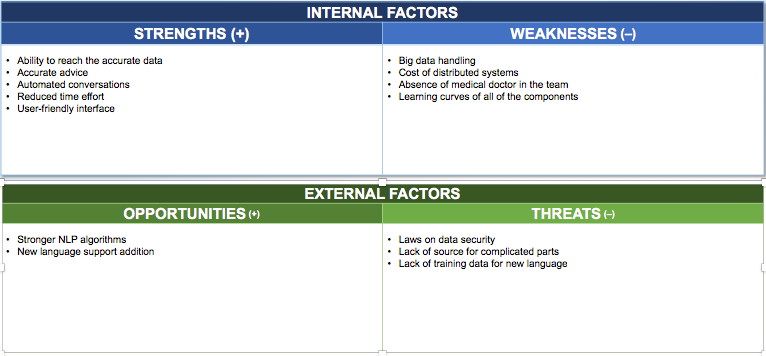
\includegraphics[width=\textwidth]{swot}
	\caption{SWOT Analysis}
	\label{swot}
\end{figure}

\section{Division of labor}

We did not have an experience in the chatbot field, and because of our lack of experience in python	tools, we did the work part in accordance with the principle of volunteering. In this context we divided the different tasks as showed on table \ref{labor}.
\begin{table}[H]
	\centering
	\begin{tabular}{|c|p{10cm}|}
		\hline
		\textbf{Group member} & \textbf{Labor} \\
		\hline
		Emirhan	Kutlu & Django back-end, ChatterBot usage and integration, Telegram chat bot programming and competitive and SWOT Analysis \\
		\hline
		Lucie Labadie & Django back-end, Multi-classifier with SciKit-learn and documentation, supervision report \\
		\hline
		Rosen Sasov & Public database search, Database architectural design and front-end \\
		\hline
	\end{tabular}
	\caption{Division of labor}
	\label{labor}
\end{table}	

Apart from these, collaborated studies and meetings	were held to decide on the method needed for diagnosis.
	
	\chapter{Project Design} %TODO

\section{Overall Architecture}

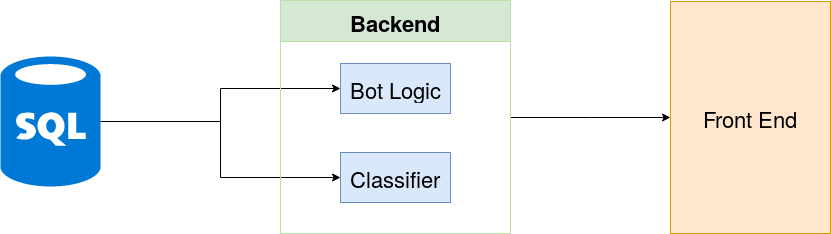
\includegraphics[height = 0.35\textheight, width = \textwidth]{Architecture}

\section{Database}

\paragraph{}
We searched for already created database with some test data that can be publicly used but we didn’t have luck. So we were forced to create our own database.\\
The database technology that we decided to use is PostgreSQL (https://www.postgresql.org/).\\
The software is open-source, which means that the source code is available at no charge. In that way if we have a need to customize or extend PostgreSQL in any way then we are able to do so with a minimum of effort, and with no attached costs.\\
PostgreSQL is available for almost every brand of Unix (34 platforms with the latest stable release), and Windows compatibility is available via the Cygwin framework.\\
And last but not least, the legendary reliability and stability of PostgreSQL.

In the area of medicine and health care it is a well known fact that there is a lot of data and many different aspects that can be considered, when taking a decision or making a diagnosis. \\
After analyzing the data itself we decided that we will choose the relational data model.
The reason is that we have a lot of data that can be dependent upon other data.\\
One obvious and clear example of that is the disease’s dependency upon symptom(s).\\
\\
Example : 
Let’s imagine that someone has the following symptoms : high temperature, fever, cough, tiredness and sweating. 
Obviously, assuming all of those symptoms we can conclude that the person might has flu. But if the person was complaining about low temperature instead of high temperature, we would most likely assume pneumonia as a state of the condition. The reason is that low temperature combined with the other symptoms is more typical for pneumonia than flu. 
Both of the examples show how we can differ our decisions one from another and how we make decision according to the chosen decision-making strategy. In other words diagnosis or more specifically final disease is the decision and the symptoms are defining our basic decision-making strategy.\\
\\
High temperature, fever, cough, tiredness, sweating → Flu\\
Low temperature, fever, cough, tiredness, sweating → Pneumonia\\
\\
Basic decision-making strategy : Symptoms\\
Decision : Diseases\\
\\
There is alternative interpretation that is valid for the upper case. The inverted case.
We can say that we can invert the roles and we will still have true logic.\\  
So we will have this :\\
\\
Flu $\rightarrow$ High temperature, fever, cough, tiredness, sweating \\
Pneumonia 		$\rightarrow$	  Low temperature, fever, cough, tiredness, sweating\\
\\
Basic decision-making strategy : Diseases\\
Decision : Symptoms\\
\\
To summarize we can say that the data dependency is bidirectional.\\
\\
Flu $\leftrightarrow$ High temperature, fever, cough, tiredness, sweating\\
\\
This is leading to the biggest problem – data handling.
In other words  we are forced to use many-to-many relationship model which is leading to a difficulties in data inserting and Big Data.

\section{Database structure and design}
\paragraph{}

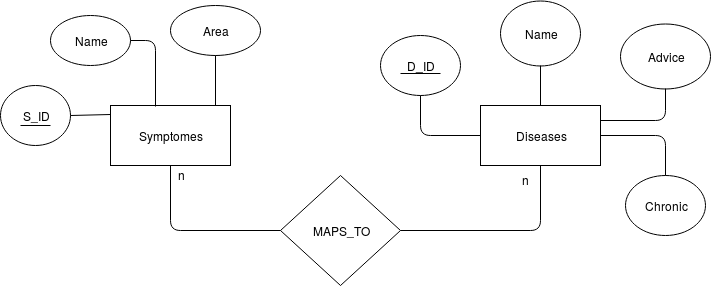
\includegraphics[height = 0.35\textheight, width = \textwidth]{DB}

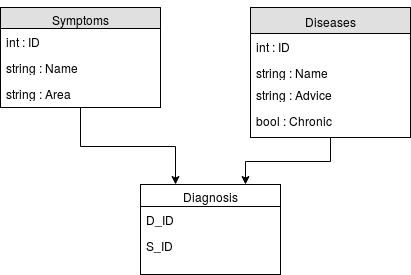
\includegraphics[height = 0.35\textheight, width = \textwidth]{UML}
\\
\\
\section{Data model}
\paragraph{}
We have 3 tables in our relational database.\\
\\
Symptoms – id, name and area which the symptom occurs. \\
Diseases – id, name, advice (medical advice if you are in that condition), chronic(boolean value used to show us if the disease is chronic or not)\\
Diagnosis – table connecting the symptoms with the diseases by ids.\\

A problem that occur our project is finding trustworthy data.\\
The data we are using is taken from http://www.mayoclinic.org/ .\\ 
The development team of the website consists of experts in the medical field. 
Physicians, scientists and other medical experts contributed to the website with their knowledge and experience. That’s the main reason why we decided to trust this website and use the data from it.   

As you can see from the diagrams the database is complicated when it’s about inserting data in it.
With the current design and structure it’s impossible to be done join between the tables for symptoms and diseases because of the data dependency. In a result while inserting data, every time we should fill the data manually in the diagnosis table in order to have the connection between every symptom and disease at the end. 
The other problem that is occurring is that the more data we are inserting the bigger becomes the diagnosis table. That means that at some point we are going to face the big data problem.


	
	\chapter{Project Implementation} 

\section{Technology choices}

\paragraph{}
When we	started	the	project,	we	aimed	to	design	a	health	bot	running	on	the	web.	When	we	started	designing	the	healthcare	bot,	we	preferred	the	Python	programming	language	in	 terms	of	resource	abundance	and	high	implementation	speed.	In	this	context,	we	decided	to	use	Django,	the	python	web	framework.	Django	is	specialized	to	make	it	easier	to	build	web	applications	with	complex	databases\cite{bib:misc:7}.	Django	is	designed	to	have	the	principles	of	reusability, modularity,	and	rapid	development	process.	For	Chatbot,	we	used	ChatterBot,	which	is	also	a	library	of	Python	language.	ChatterBot	is	designed	for	the	development	of	bots	that	can	communicate	with	the	user	through	an	educatable	automated	dialogue\cite{bib:misc:8}.	Finally,	we	used	Scikit-Learn,	a	python	machine	learning	package,	to	get	the	symptoms	out	of	the	input.	
\paragraph{}
Due	to	the	lack	of	available	data,	we	had	to	decide	late	on	the	database	architecture.	Due	to	this	reason,	we	delayed	the	construction	of	the	application	with	django,	which	is	based	on	modeling	in	the	database.	At	the	same	time,	the	deficiencies	in	ChatterBot	and	django	integration	and	the	size	of	the	solution	learning	curve	pushed	us	to	change	technology.	For	this	reason,	we	decided	to	develop	a	Telegram	bot	as	a	tool	that	we	can	focus	only	on	bot	training\cite{bib:misc:9}.	Telegram	is	an	open	source	instant	messaging	application.	

\paragraph{}
In order to create the classifier we decided to use \textit{SciKit-learn}\cite{bib:misc:2} a python module easy to use and with wide customization possibilities. To test and visualize the results of the classifier two other tools were used : \textit{Jupyter}\cite{bib:misc:3} and \textit{matplotlib}\footnote{A python library to display plots}

\paragraph{}
The database technology that we decided to use is \textit{PostgreSQL}\cite{bib:misc:1}.
\paragraph{}
The software is open-source, which means that the source code is available at no charge. In that way if we have a need to customize or extend PostgreSQL in any way then we are able to do so with no attached costs.
\paragraph{}
PostgreSQL is available for almost every version of Unix (34 platforms with the latest stable release), and Windows compatibility is available via the Cygwin framework.
\paragraph{}
And last but not least, the legendary reliability and stability of PostgreSQL.

\section{Natural Language Recognition}

\subsection{Classifier implementation}

\paragraph{}
In	order	to	process	the	symptom	from	the	user	as	a	meaningful	message	text,	we	treat	each	symptom	stored	in	our	database	as	a	class.	In	this	way,	we	can	see	if	the	input	from	the	user	is	a	symptom	and	if	it	is	a	symptom	which	symptom	it	is.	We	created	some	training	data	for	each	symptom.	At	this	point,	we	can	catch	the	same	complaint	being	expressed	in	different	words.	For	example,	when	a	user	says	"I	have	pain	in	my	head"	instead	of	"I	have	a	headache",	we	have	a	chance	to	catch	that	the	symptom	is	actually	a	headache.	

\paragraph{}
In order to understand the symptom the user enters in as an input, a classifier is used. The dataset is composed of the symptoms and different expressions of them, per example the pair \texttt{headache : my head hurts}.

\paragraph{}
First of all, as the classes are known, a supervised method is to be used. In natural language processing the Support Vector Machine (SVM)\cite{bib:misc:6} is well known for its efficiency on supervised problems. So it has been decided to use this method. 

\begin{figure}[H]
	\centering
	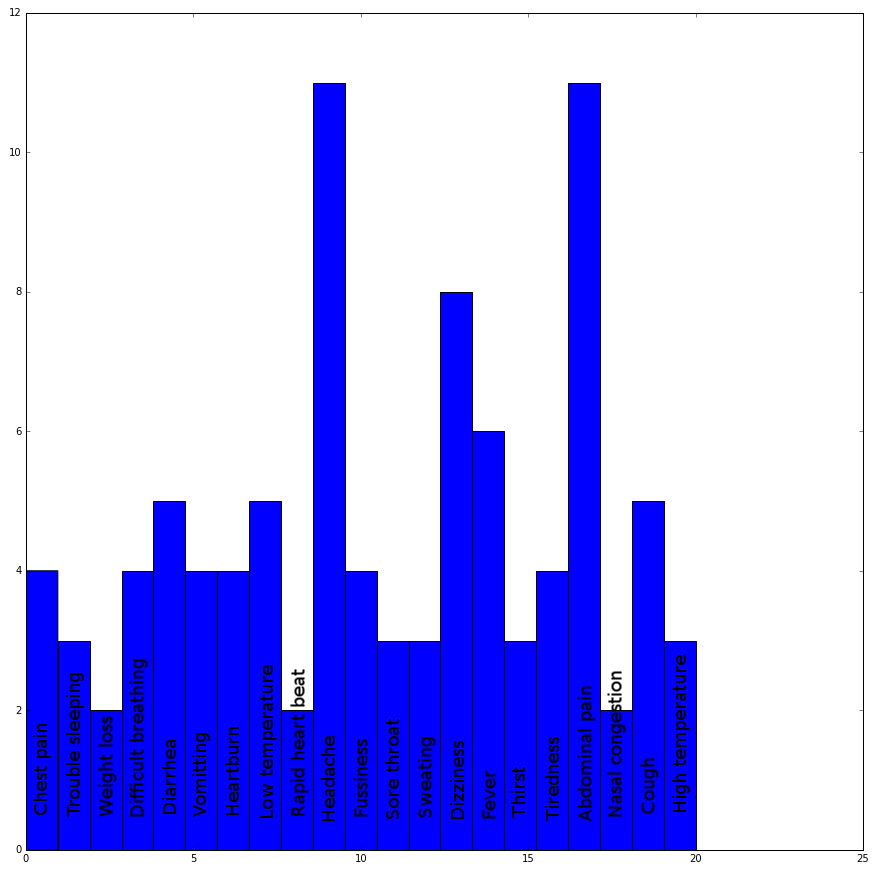
\includegraphics[height=10cm]{classifier_classes_repartition}
	\caption{Data repartition of the dataset}
	\label{dataset}
\end{figure}

\paragraph{}
Different tests has been done to obtain a good classifier. Two different implementations of SVM has been used. First the \texttt{multi-class one-against-one classification}\footnote{If $n_class$ is the number of classes, then $n_class * (n_class - 1) / 2$ classifiers are constructed and each one trains data from two classes.} with different \texttt{aggregation shapes}\footnote{To provide a consistent interface with other classifiers, the results of the “one-against-one” classifiers can be aggregate using different decision function of shape} then the \texttt{multi-class one-vs-the-rest classification}\footnote{If $n_class$ is the number of classes, then $n_class$ classifiers are constructed. If there are only two classes, only one model is trained} with a linear kernel\cite{bib:misc:5}. The main difference is that solving the optimization problem for a linear kernel is much faster than for non-linear with a negligible loss of predictive performance\cite{bib:article:1}.

\paragraph{}
In order to compare the different classifier created, we used confusion matrix. First the classifiers has been tested on the training data then the best one on a test set\footnote{Containing values that are not in the training set}. 
\newpage
\begin{multicols}{2}
	\begin{figure}[H]
		\centering
		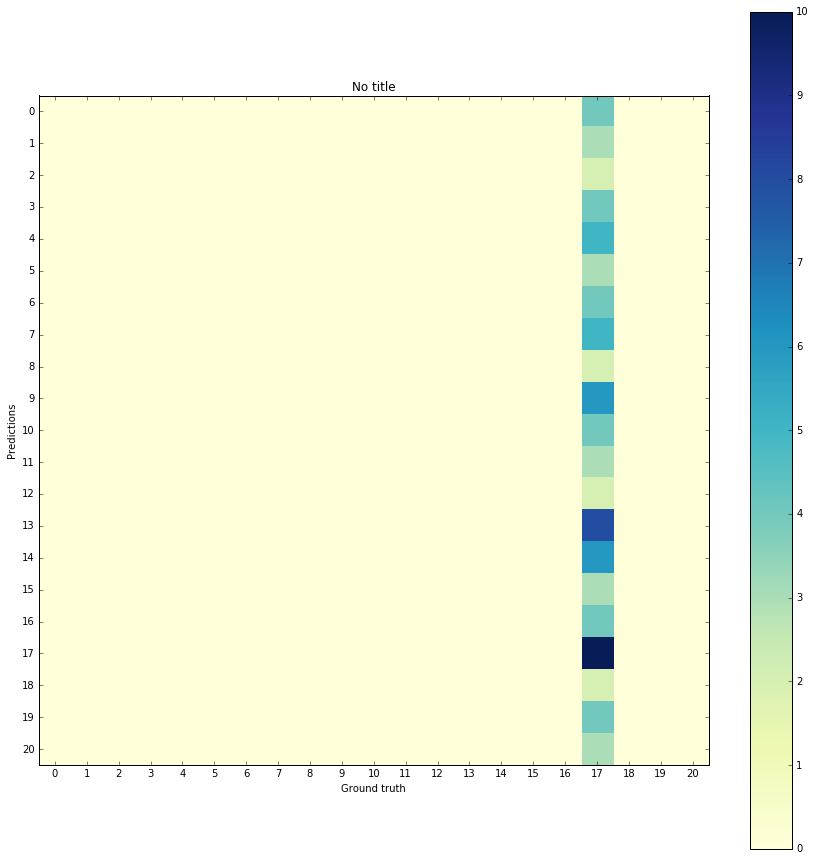
\includegraphics[width=0.4\textwidth]{classifier_svm}
		\caption{Confusion matrix for SVM}
		\label{svm}
	\end{figure}

	\begin{figure}[H]
		\centering
		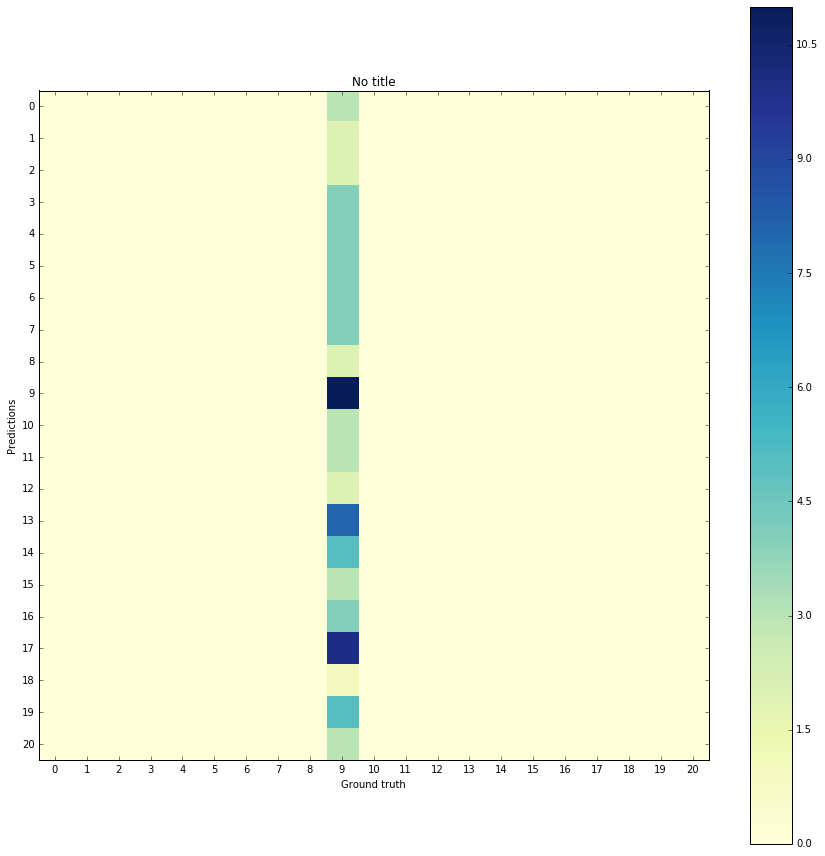
\includegraphics[width=0.4\textwidth]{classifier_svm_ovo}
		\caption{Confusion matrix for SVM using ovo aggregation function}
		\label{svm_ovo}
	\end{figure}
	
\end{multicols}

\begin{multicols}{2}
	\begin{figure}[H]
		\centering
		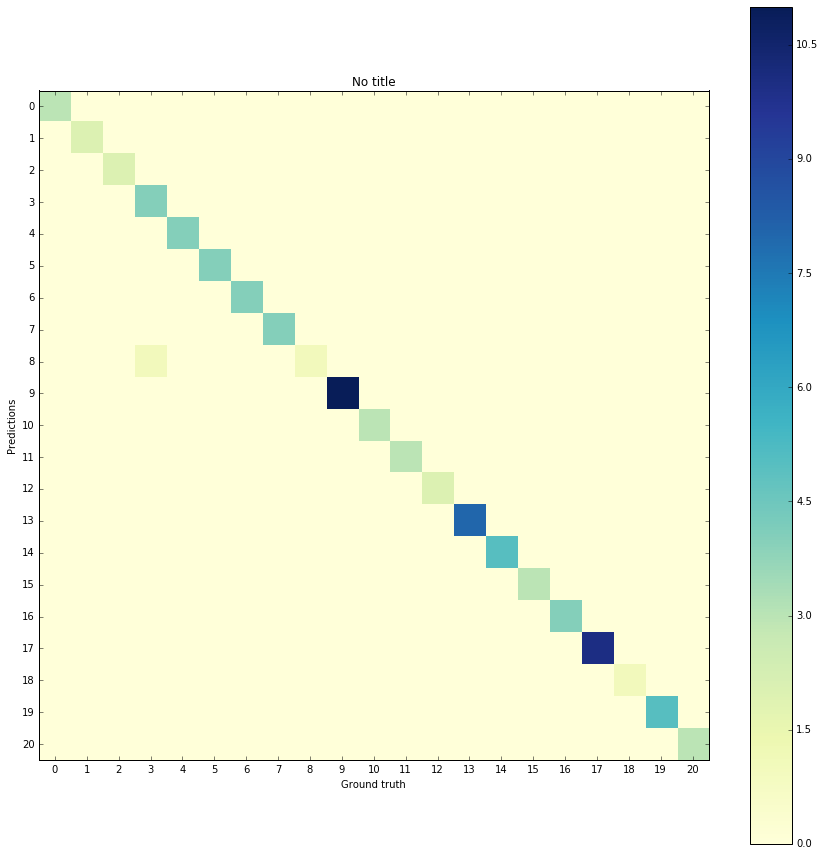
\includegraphics[width=0.4\textwidth]{classifier_svm_linear}
		\caption{Confusion matrix for linear SVM}
		\label{svm_linear}
	\end{figure}
	\begin{figure}[H]
		\centering
		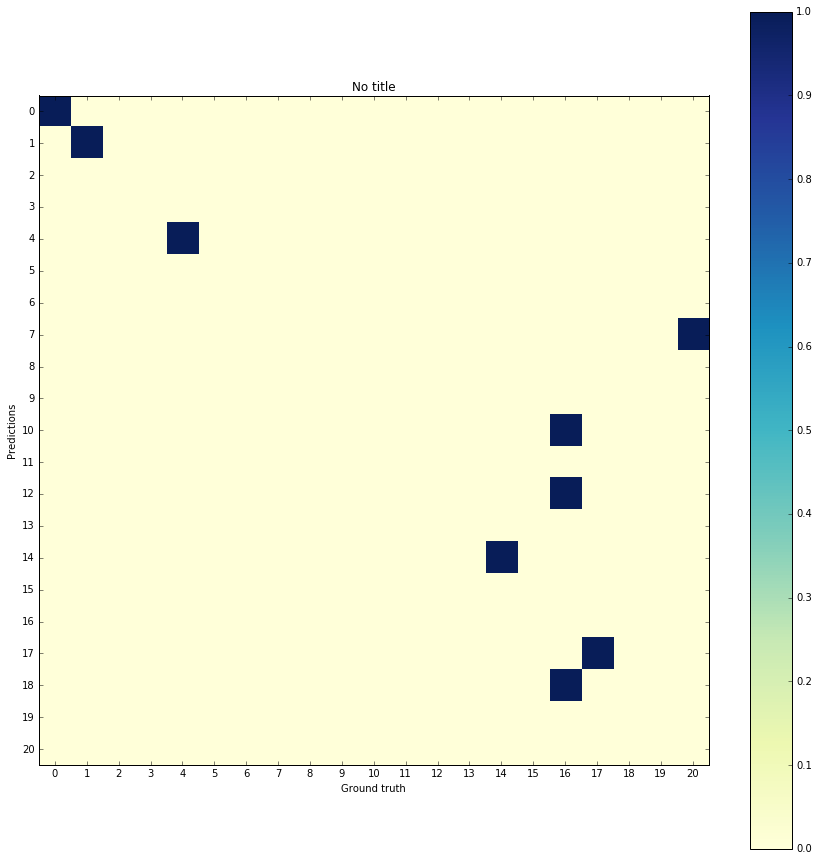
\includegraphics[width=0.4\textwidth]{classifier_svm_linear_test}
		\caption{Confusion matrix for linear SVM on test set data}
		\label{svm_test}
	\end{figure}
\end{multicols}

So the linear SVM has been chose, for its results better than the two other attempts. 

\subsection{Review on results}

The chosen classifier present only 0.5 accuracy. This middling performance is mainly due to the small size of the dataset. In order to improve the results several solution can be implemented.
\begin{itemize}
	\item Data processing: remove meaningless words (like "in", "my"...) change verbs by their infinitive form.
	\item Use of $n-gram$. This technique consist in using group of words to define a concept instead of words alone. First we look at one word, then 2 and 3 up to $n$.
\end{itemize}

\section{Interface}

\paragraph{}
We	have	the	opportunity	to	use	and	customize	the	telegram	chat	interface.	If	the	user	is	only	asked	to	make	a	selection	rather	than	enter	the	data,	the	options	can	be	presented	easily.	

\begin{figure}[H]
	\centering
	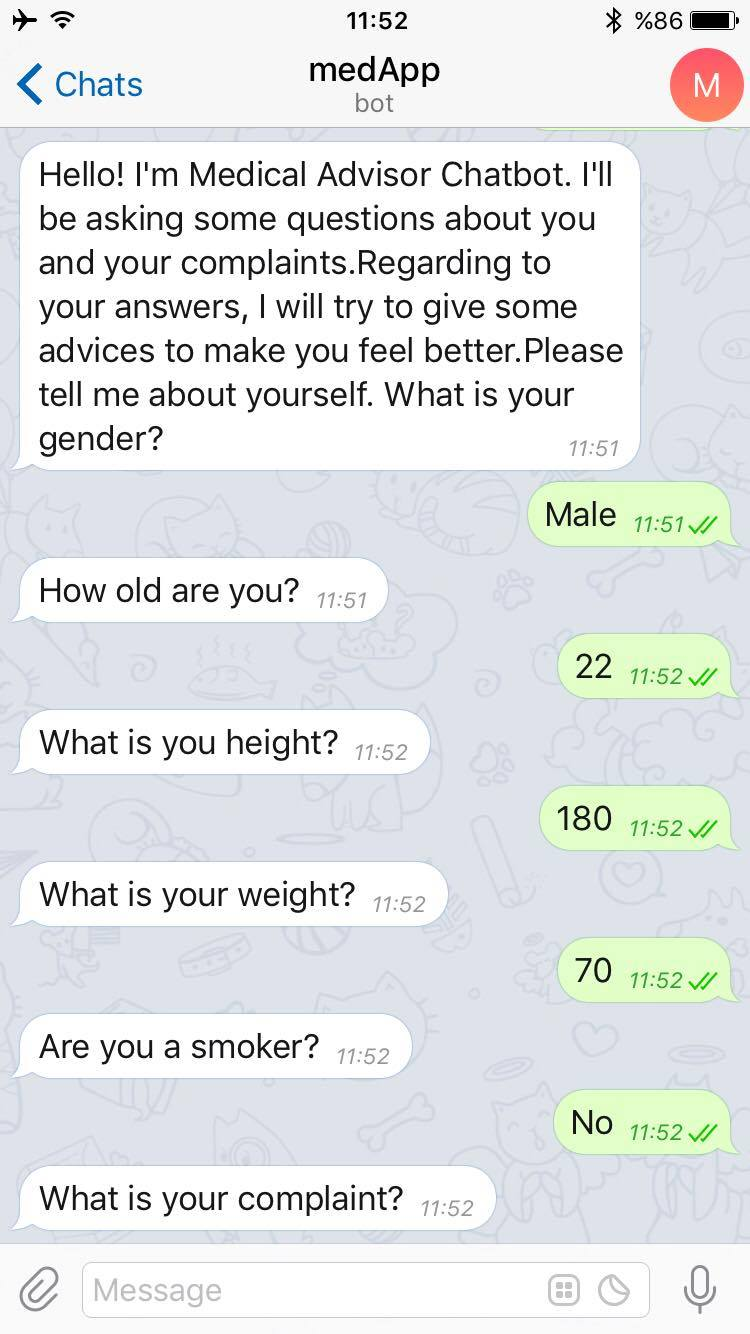
\includegraphics[height=10cm]{screenshot}
	\caption{Bot interface}
	\label{screen}
\end{figure}

\section{Questions logic}

\begin{figure}[H]
	\centering
	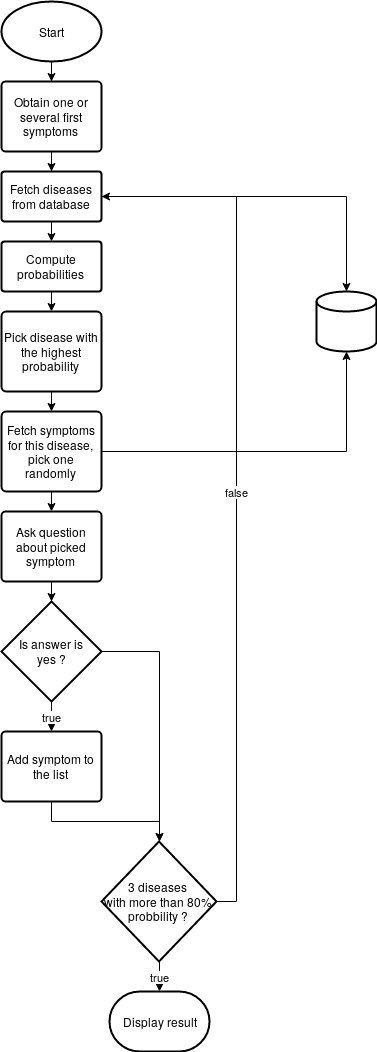
\includegraphics[height=0.9\textheight]{flow_chart_questions}
	\caption{Control flow graph showing the questions logic}
	\label{cfg_logic}
\end{figure}

\section{Decision making}

\paragraph{}
First,	we	get	personal	information	from	the	user	such	as	gender,	height,	weight,	etc.,	to	use	to	calculate	the	diagnosis	later.	We	then	take	the	user's	complaint	and	determine	which	of	the	symptoms	in	the	data	base	is	pointing	to.	We	find	diseases	with	this	symptom	by	searching	the	incoming	symptom	database.	Then,	we	ask	other	symptoms	of	these	diseases	whether	the	user	has	it.	If	the	patient	gives a	yes	response to	this	question,	we	increase the score	of the	diseases	that	the	symptom	belongs	to.	When	the	questions	are	over,	we	tell	the	patient	what	the	patients condition might be	and	we	give	advice	for	the	treatment.	We	then	aim	at	evaluating	personal	data	so	as	to	minimize	any	possible	equality	between	diseases	after	scoring.	In	this	project,	we	prepared	the	database	for	ourselves,	so	we	included	close	health	problems	similar	to	each	other	in	our	data	set.	At	this	point,	we	think	that	we	can	see	the	results	of	the	scoring	in	a	healthier	way.	
	
	\chapter{User and competitive Analysis} 

\section{User Analysis}

\paragraph{}
Due	to	health	data	pollution	on	the	Internet,	it	is	very	difficult	for	people	to	access	reliable	healthcare	data.	Because	of	the	potential	panic	of	data	pollution	and	the	inability	to	respond	to	every	incoming	question,	customization	is	essential	to	respond	to	this	need.	In	this	context,	the	main	target	audience	for	this	application	is	any	user	who	needs	information	about	health.	The	advantages	of	the	application	can	be	listed	as	follows:
\begin{itemize}
	\item Reliable	health	information	data;
	\item Accurate	treatment	for	the	complaint;
	\item Reduced	time	effort;
	\item User-friendly	interface.
\end{itemize}

\section{Competitive	Analysis	}

\paragraph{}
There	are	four	successful	projects	in	this	area,	three	from	the	UK	and	one	from	the	People's	Republic	of	China.		

\paragraph{Your	Md.:}This	application,	which	has	been	on	the	market	with	the	support	of	the	UK	Ministry	of	Health,	draws	symptoms	from	the	user's	text	and	asks	for	more	detailed	questions.	As	a	result	of	the	estimation,	detailed	information	is	given	about	prominent	diseases	and	treatments.	

\paragraph{Babylon	Health:}This	UK-based	application	is	also	collecting	data	similar	to	your	Md.	In	addition,	there	is	the	possibility	of	paid	consultation	to	a	doctor	by	voice	or	video.	

\paragraph{Ada	Health:}Unlike	the	other	two	applications,	the	user	selects	a	symptom	from	a	search	made	with	the	help	of	key	words,	not	the	text,	and	asks	users	questions	based	on	them.	At	the	same	time,	the	application	has	the	ability	to	train	itself	by	storing	user	data.	

\paragraph{Baidu	Melody:}The application	claims	that	Baidu	developers	have	succeeded	in	creating	a	powerful	medical	assistant	with	advanced	depth	learning	and	natural	language	processing	skills.	However,	this	practice	can	only	be	used	on	the	borders	of	the	People's	Republic	of	China.	

Unlike	other	applications	in	our	project,	what	we	want	to	do	is	to	get	all	of	the	complaints	from	the	entered	text,	reduce	the	time	to	diagnose	and	increase	the	accuracy.			

	
	\addcontentsline{toc}{chapter}{Conclusion}
	\chapter*{Conclusion}
	\paragraph{}
	%TODO
	Here comes the conclusion
	
	%%if needed part
	
	%\input{appendix}
	
	%\bibliographystyle{plain}
	%\bibliography{biblio}
	
\end{document}  
